\documentclass[12pt,a4paper]{report}
\usepackage[brazilian]{babel}
\usepackage[utf8]{inputenc}
\usepackage[T1]{fontenc}
\usepackage{amsmath,amsthm,amsfonts,amssymb,textcomp}
%\usepackage{latexsym}
\usepackage{graphicx}
\graphicspath{{figuras}}
\usepackage{subfigure}
\usepackage{float}
\usepackage{longtable}
\usepackage{color}
\usepackage{epstopdf}
\usepackage{pdflscape}
\usepackage[breaklinks=true]{hyperref}
\usepackage[comma,authoryear]{natbib}
%\usepackage[nonumberlist]{glossaries}
\usepackage{arydshln}
\usepackage{footnote}
\usepackage{longtable}
\usepackage[small,bf,singlelinecheck=off]{caption}
\usepackage[left=3cm,right=2cm,top=3cm,bottom=2cm]{geometry}
%\usepackage[alf]{abntcite}

%%% newcommand %%%%%%%%%%%%%%%%%
\newcommand{\PE}{Perkin-Elmer }
\newcommand{\BC}{Boller \& Chivens }

\newcommand{\degr}{\ensuremath{^{\circ}}}%                    % degree symbol:  °
\newcommand{\arcmin}{\ensuremath{^{\prime}}}%                    % degree symbol:  °
\newcommand{\arcsec}{\ensuremath{^{\prime\prime}}}%                    % degree symbol:  °
\newcommand{\fs}{\mbox{\ensuremath{.\!\!^s}}}
\newcommand{\farcm}{\mbox{\ensuremath{.\mkern-4mu^\prime}}}%    % fractional arcminute symbol: 0.'0
\newcommand{\farcs}{\mbox{\ensuremath{.\!\!^{\prime\prime}}}}%  % fractional arcsecond symbol: 0.''0
\newcommand{\fdg}{\mbox{\ensuremath{.\!\!^\circ}}}%             % fractional degree symbol:     0.°0



%\makeglossaries

\makeatletter
\renewcommand\chapter{\thispagestyle{plain}
                \global\@topnum\z@
                \@afterindentfalse
                \secdef\@chapter\@schapter}
\makeatother


\makeatletter
\renewcommand{\@makechapterhead}[1]{%
\vspace*{50 pt}%
{\setlength{\parindent}{0pt} \raggedright \normalfont
\bfseries\Huge\thechapter.\ #1
\par\nobreak\vspace{40 pt}}}
\makeatother

\renewcommand{\thesection}{\arabic{section}}

%\newglossaryentry{Offset}{name={Offset}, description={Diferença entre a posição obtida pela redução da observação e a posição dada pela efeméride}}
\newglossaryentry{OPD}{name={OPD}, description={Observatório do Pico dos Dias - Brasópolis, MG}}
\newglossaryentry{LNA}{name={LNA}, description={Laboratório Nacional de Astrofísica - Itajubá, MG}}
\newglossaryentry{OHP}{name={OHP}, description={Observatoire Haute Provence - Saint-Michel-l'Observatoire, França}}
\newglossaryentry{RA}{name={RA}, description={Sigla para Ascensão Reta ($ \alpha $)}}
\newglossaryentry{DEC}{name={DEC}, description={Sigla para Declinação ($ \delta $)}}
\newglossaryentry{Anomalia Verdadeira}{name={Anomalia Verdadeira}, description={Ângulo formado entre o Periastro e a posição instantânea do objeto na órbita centrado no planeta e contada na direção do movimento orbital}}
\author{Altair Ramos Gomes Júnior}
\title{Ocultações Estelares por Satélites Irregulares}
\begin{document}

\maketitle

\pagestyle{headings}

\section{Introdução} \label{Chap:Intro}

\indent \indent O estudo de objetos como objetos trans-Neptunianos (TNOs), Centauros e Satélites Irregulares nos ajudam a compreender a formação e evolução do Sistema Solar Exterior. Nesta região distante do Sol, de baixas temperaturas, objetos principalmente de tamanho relativamente pequeno, e mais dispersos no espaço, provavelmente sofreram muito pouca diferenciação, seja por mecanismos internos, seja por choques com outros corpos, comparados a objetos formados mais próximos do Sol.

Por serem corpos asteroidais localizados de forma dispersa além da órbita de Netuno, considera-se que os TNOs guardam estruturas e composições relativamente inalteradas em relação a sua época de formação, constituindo-se assim em corpos de prova de grande valor para o estudo da origem do Sistema Solar, ao menos para essa região exterior.

Tirando Plutão, o primeiro TNO foi descoberto há pouco mais de 20 anos \citep{Jewitt1993}. Por isso, as propriedades básicas desta população ainda não estão inteiramente estabelecidas, como a distribuição de tamanhos, composição, estruturas internas.

Atualmente, é aceito que TNOs tenham sido formados nas partes mais internas do Sistema Solar. Eles teriam então sido colocados em suas posições atuais devido a troca de momento angular entre os planetas e planetésimos quando da migração dos planetas gigantes. A evolução se deu de tal forma que a passagem dos planetesimais e planetas por zonas de ressonância de movimento médio redefiniu as órbitas desses corpos \citep{Tsiganis2005}.

Muitos dos objetos que pertenciam ao cinturão de Kuiper primordial acabaram sendo enviados pela interação com os planetas gigantes para as partes mais internas do Sistema Solar. Alguns podem ter sido capturados pelos planetas criando a população de satélites irregulares ou satélites externos \citep{Nesvorny2007}, troianos \citep{Morbidelli2005} ou até mesmo para o cinturão principal de asteroides como proposto para Ceres por \cite{McKinnon2012}. Estudar esses objetos é de grande importância para entender a evolução do Sistema Solar.

Os satélites irregulares dos planetas gigantes são menores que os regulares, possuindo órbitas mais excêntricas, inclinadas e distantes. Na maioria dos casos, essas órbitas são retrógradas. Devido a suas configurações orbitais, é amplamente aceito que estes objetos foram capturados nos estágios iniciais da formação do Sistema Solar \citep{Sheppard2003}. Figura \ref{Fig:sat-conf} resume as características orbitais dos satélites irregulares de Júpiter e Saturno.

\begin{figure}[h]
\begin{centering}
\subfigure[Satélites de Júpiter]{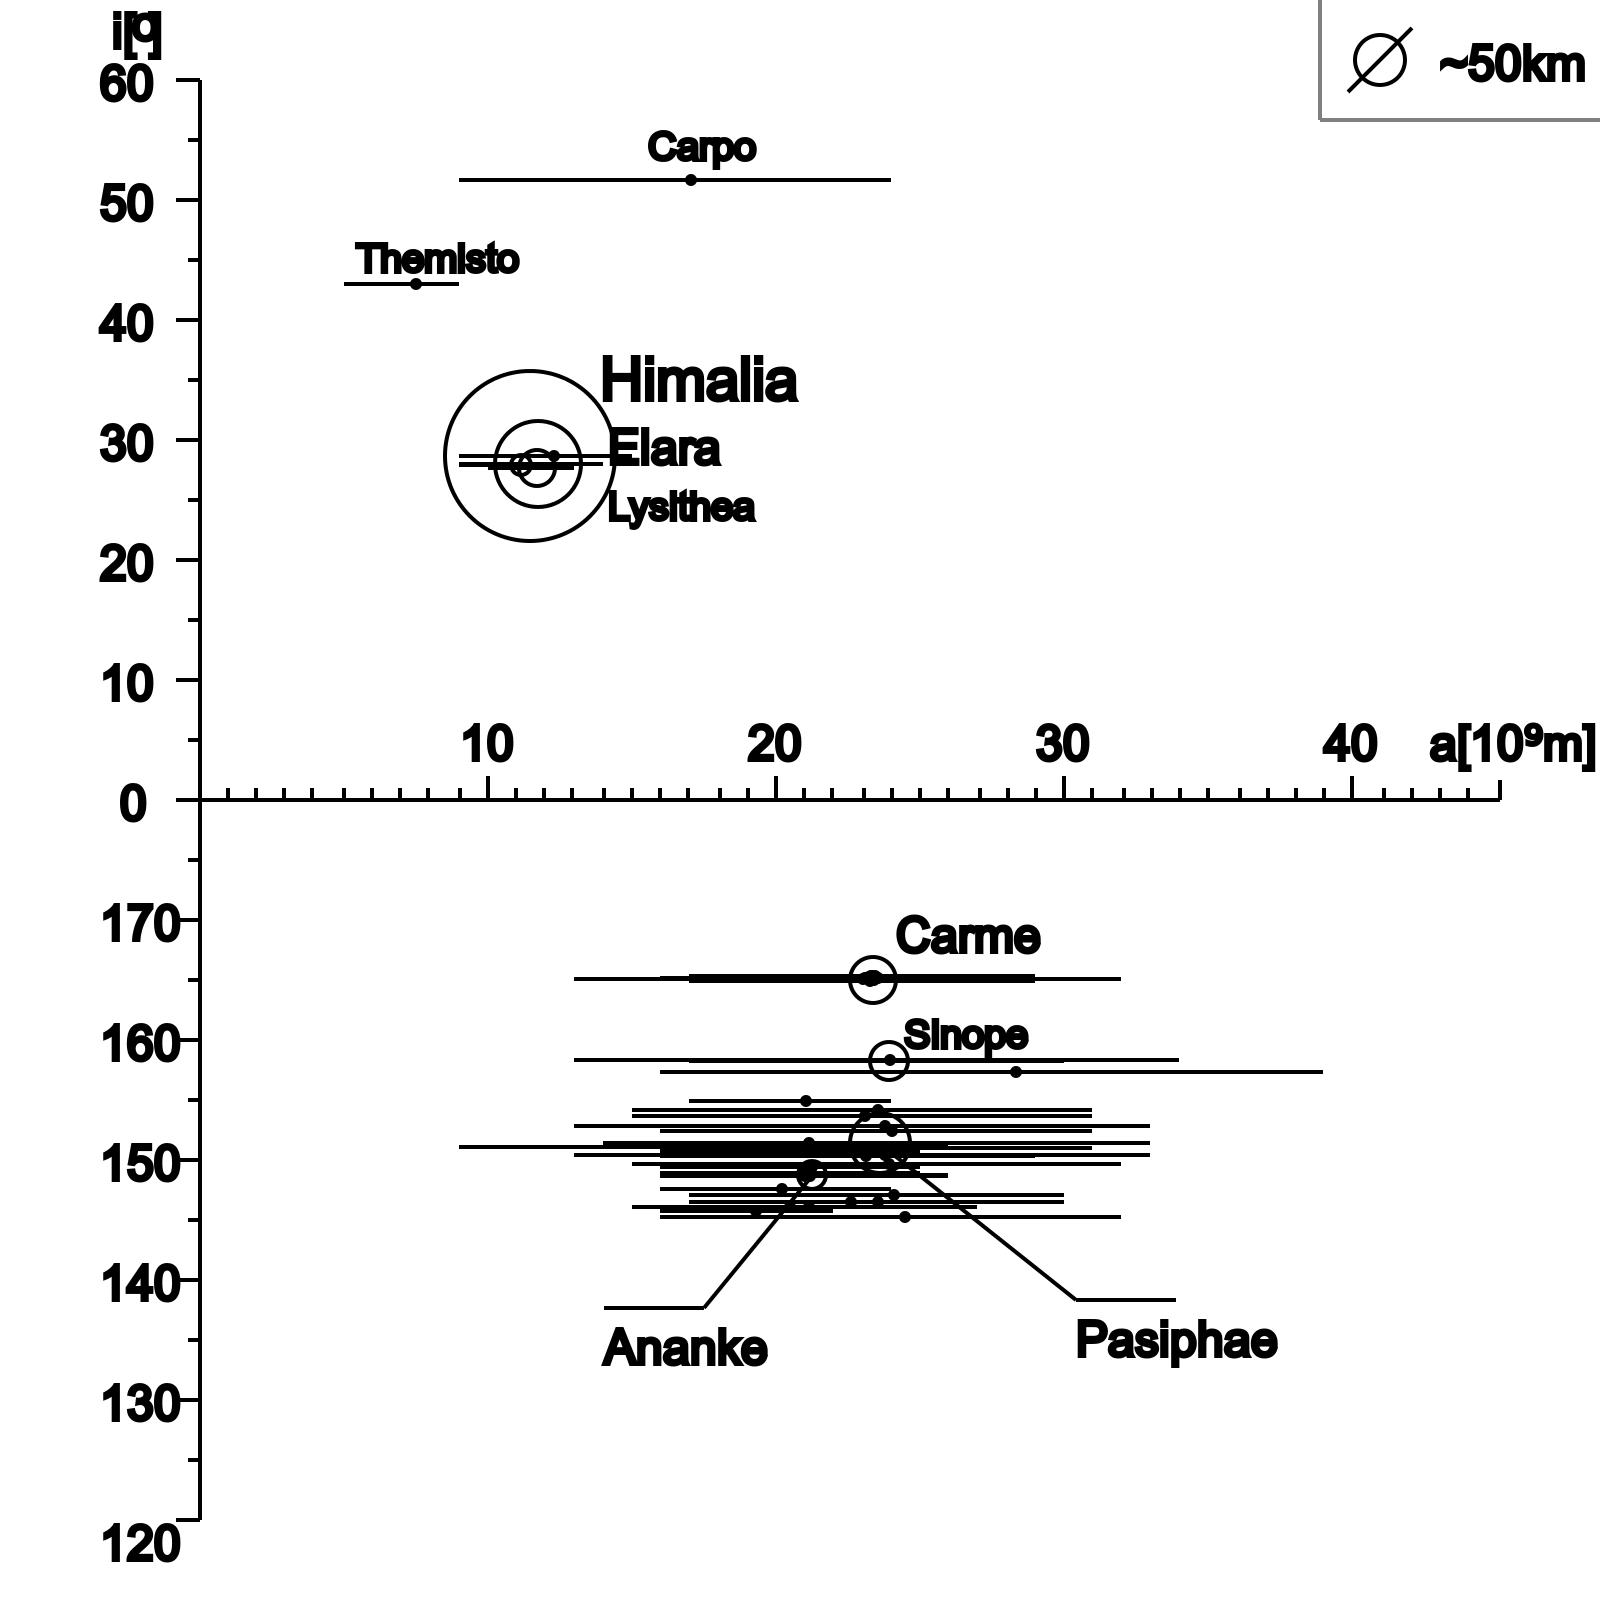
\includegraphics[scale=0.13]{figuras/Jupiter2.jpg}\label{Fig:sat-jup} }
\subfigure[Satélites de Saturno]{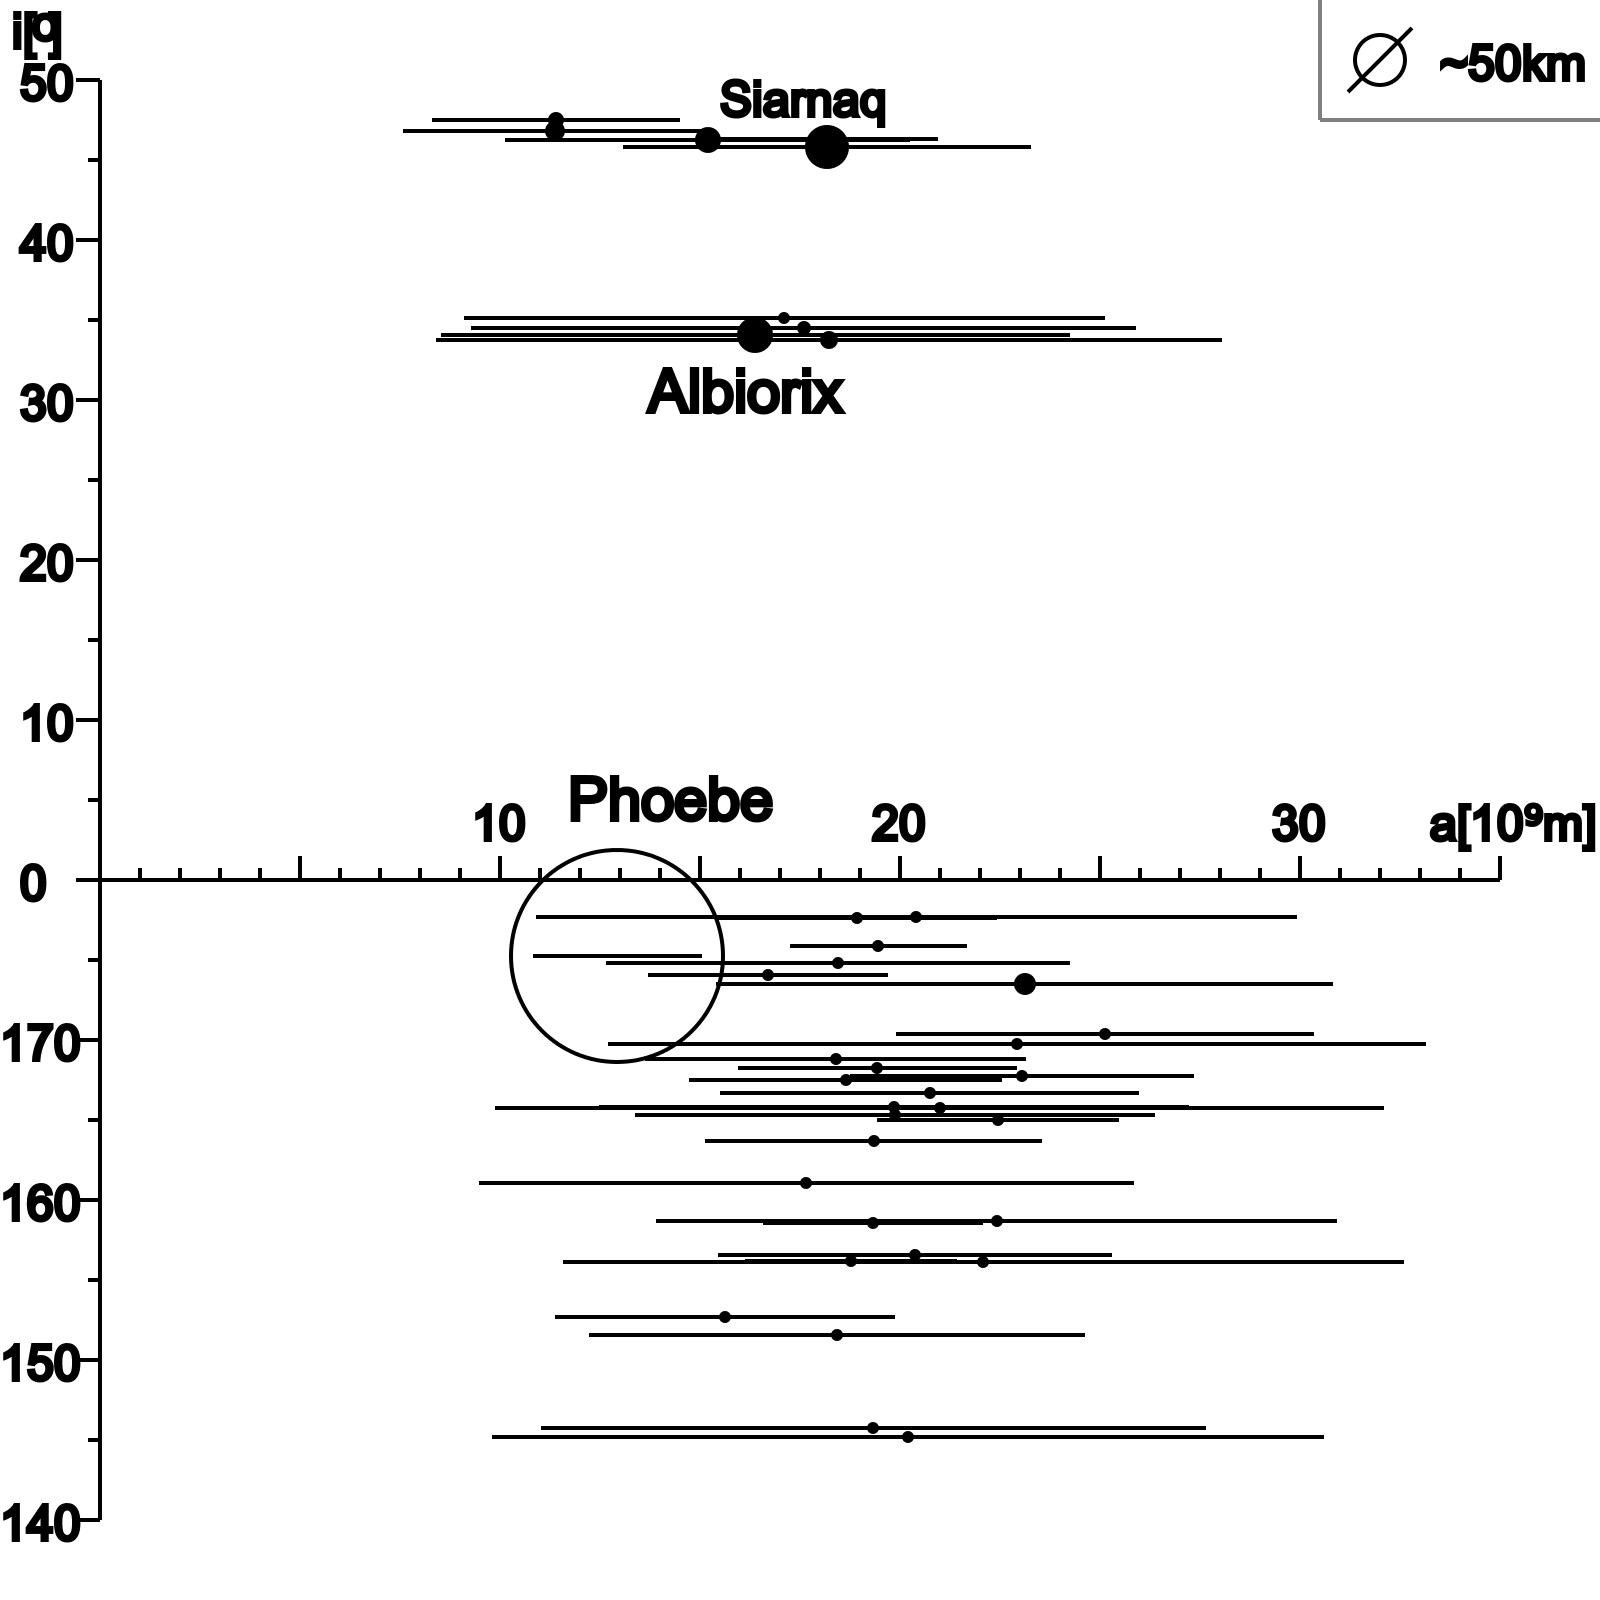
\includegraphics[scale=0.13]{figuras/Saturno2.jpg}\label{Fig:sat-sat} }
\caption{Esquema ilustrativo das órbitas dos satélites irregulares: a escala vertical se refere à inclinação em graus da órbita dos satélites em relação ao planeta; a escala horizontal é a distância em milhões de Km ao planeta; as linhas representam a variação de distância do satélite ao planeta durante o período orbital; os círculos são os tamanhos relativos dos satélites.(baseado em dados obtidos do JPL, via site Horizons).
\label{Fig:sat-conf}}
\end{centering}
\end{figure}

Por serem pequenos, eles são pouco brilhantes e só foram descobertos no último século\footnote{Website: \url{http://ssd.jpl.nasa.gov/?sat\_discovery}}. Até o momento, apenas os planetas Júpiter, Saturno, Urano e Netuno possuem satélites irregulares conhecidos, embora a possibilidade de que outros corpos, como Plutão, possuam tais satélites não são nulas \citep{Michaely2017}. Devido a isso, as menções a "satélites irregulares" presentes neste texto referem-se aos satélites irregulares dos planetas gigantes.

%Existem alguns mecanismos de captura de objetos por planetas gigantes propostos na literatura. Há o Arrasto Gasoso na nebulosa circumplanetária primordial \citep{Sheppard2005} onde o movimento do objeto seria afetado pelo gás e sua velocidade diminuiria até que fosse capturado pelo planeta. Outro mecanismo se chama captura pull-down \citep{Sheppard2005}, onde a massa do planeta aumentaria enquanto o objeto estivesse temporariamente capturado.

%Um mecanismo baseado no modelo de Nice \citep{Morbidelli2005, Tsiganis2005, Gomes2005} foi proposto por \cite{Nesvorny2007} e, especificamente para Júpiter, por \cite{Nesvorny2014}. Durante a instabilidade do Sistema Solar primordial, ocorreram encontros entre os planetas externos. Nesses encontros planetários poderia haver troca de energia e momento angular entre os planetas e os objetos próximos tornando possível a captura de um corpo irregular por um planeta gigante. Nesse cenário, a taxa de sobrevivência de satélites anteriores ao LHB (Bombardeamento Pesado Tardio\footnote{"Late Heavy Bombardment", em inglês}) é muito pequena.

%Um terceiro mecanismo importante é a captura através de interações colisionais \citep{Sheppard2005}. Uma colisão entre dois corpos pequenos dentro da esfera de Hill do planeta poderia gerar objetos fragmentados e a energia dissipativa poderia ser tal que alguns desses objetos seriam capturados.

%Alguns desses objetos formam grupos dinâmicos com elementos orbitais semelhantes, chamados famílias, similar às famílias encontradas no Cinturão Principal de Asteroides. Essas famílias podem ter sido criadas a partir de um corpo pai que se fragmentou por colisões com cometas ou outros asteroides \citep{Nesvorny2004}. Colisões com cometas tem uma probabilidade maior de ocorrer durante o Bombardeamento Pesado Tardio (LHB) \citep{Gomes2005}.

%\cite{Nesvorny2003} estudou as taxas de colisões entre satélites irregulares e concluiu que alguns satélites podem ter sido removidos por colisão com um satélite maior. A taxa de colisão entre os satélites do grupo de Himalia (Himalia, Elara, Lysithea and Leda, principalmente), por exemplo, foi encontrado como sendo maior que 1 durante a idade do Sistema Solar sugerindo que sua estrutura atual foi originada por colisão satélite-satélite.

%Para Phoebe, materiais ejetados de sua superfície causadas por impactos poderiam evoluir devido ao arrasto de Poynting-Robertson e colidir com Iapetus causando a grande variação de albedo observada no satélite \citep{Nesvorny2003}. De fato, a sonda \textit{Cassini} detectou em Phoebe uma característica de absorção em 2.42 $\mu m$, provavelmente combinações de CN, que foi também detectada no lado escuro de Iapetus \citep{Clark2005}.

Se esses objetos foram capturados, permanece a pergunta de onde eles vieram. \cite{Clark2005} mostraram a partir de espectroscopia da Cassini que Phoebe tem uma superfície provavelmente coberta por material do Sistema Solar externo e \cite{Grav2003} mostraram que os satélites de grupo prógrado de Júpiter Himalia tem cores cinzas implicando que suas superfícies são similares a asteróides tipo C. Nesse mesmo trabalho, o grupo retrógrado de Júpiter Carme foi encontrado como tendo cores superficiais semelhantes à asteroides tipo D como a família de Hilda ou famílias de troianos, enquanto J13 Kalyke tem uma cor mais avermelhada como centauros ou objetos trans-Netunianos (TNOs).

Para os satélites de saturno, \cite{Grav2007} mostraram através de suas cores e inclinações espectrais que esses satélites contêm uma fração mais ou menos igual de objetos semelhantes a asteroides tipo C, P e D, mas S22 Ijiraq é um pouco mais avermelhado que objetos tipo D. Esses trabalhos sugerem origens diferentes para os satélites irregulares.

Dentre os satélite irregulares, poucos são aqueles que possuem medidas de seus parâmetros físicos. Apenas Himalia, Phoebe e Nereida foram observados por sondas, apesar de não serem medidas ideais, já que foram alvos de oportunidade. A sonda \textit{Cassini} observou Himalia em 2000 ao passar próximo a Júpiter e obteve o tamanho de Himalia com um erro médio de 10 km \citep{Porco2003}.

Em 2004, a \textit{Cassini}, aproximando-se de Saturno, observou Phoebe em alta resolução obtendo um erro médio na medida de seu tamanho de 0.7 km \citep{Thomas2010}. Por fim, Nereida foi observado em 1989 pela sonda \textit{Voyager II} e seu tamanho foi obtido com um erro de 25 km \citep{Smith1989}. Para outros satélites irregulares de Júpiter, seus tamanhos foram estimados por \cite{Rettig2001} impondo um albedo de 4\% com a justificativa de que esse valor é um albedo nominalmente utilizado para objetos do Sistema Solar Externo.

\cite{Grav2015}, utilizando observações em infra-vermelho obtidos dentro do projeto WISE, da NASA, inferiu os tamanhos de 11 satélites irregulares de Júpiter e 3 de Saturno. Os diâmetros médios obtidos têm erros da ordem de 1 km para os satélites de Júpiter e 5 km para os de Saturno. Porém, como se espera para objetos desses tamanhos, eles não devem possuir formatos esféricos e serem craterizados.

Um método que tem se mostrado eficiente para a obtenção de características físicas de objetos distantes a partir de observações de solo é o método de ocultações estelares. Essa técnica proporciona medidas tão precisas que são apenas superadas por medidas oriundas de sondas, in loco. Porém, devido às escalas envolvidas nessa técnica, um grande trabalho de predição e atualização desses eventos deve ser feito para gerar resultados satisfatórios.

Como previsto por \cite{GomesJunior2016}, em 2018 Saturno irá atravessar o plano da Galáxia, aumentando em mais de 20 vezes a probabilidade de uma ocultação estelar. O mesmo para Júpiter, em 2019-2020. Com a publicação da primeira versão do catálogo Gaia em Setembro de 2016 e a segunda versão prevista para Abril de 2018, a posição das estrelas no céu não será mais um problema. Restará, contudo, a melhoria no conhecimentos das órbitas dos satélites irregulares.

O objetivo do pós-doc proposto é, portanto, composta de três etapas: a observação contínua dos satélites irregulares e obtenção de posições de alta precisão através de astrometria de campo (Seção \ref{Sec:astrometria}); a integração numérica das órbitas desses satélites utilizando posições antigas e novas, bem como pesando essas posições de forma adequada (Seção \ref{Sec:Integ}); e, por fim, gerenciar campanhas de observações de ocultações por satélites irregulares, nos mesmos moldes como tem sido feito para ocultações por TNOs e que deram ótimos resultados, e, fortuitamente, observar tais ocultações e publicar seus resultados (Seção \ref{Sec:Occ}).

\section{Astrometria} \label{Sec:astrometria}

\indent \indent O primeiro satélite irregular a ser descoberto foi Phoebe, satélite de Saturno, em 1898. Porém, até 1997, apenas uma dezena de satélites haviam sido descobertos, sendo 8 de Júpiter, 1 de Saturno e 1 de Netuno \citep{Sheppard2005}. O número de satélites irregulares descobertos, porém, aumentou consideravelmente com o início da era dos grandes surveys, nos anos 2000 \citep{Sheppard2003}. Atualmente, se conhece quase 100 satélites irregulares, sendo metade deles orbitando Júpiter.

Devido a serem objetos tão recentes e pouco brilhantes, poucas observações foram feitas até o momento. Por exemplo, os modelos orbitais mais recentes para os satélites irregulares de Júpiter, publicados por \cite{Brozovic2017}, fazem uso de menos cem observações distribuídas em dez anos para a maioria dos satélites. Apenas 6 possuem mais que mil observações.

O Grupo de Astrometria do Rio de Janeiro tem feito contínuas observações de diversos objetos do Sistema Solar no Observatório do Pico dos Dias (OPD). Dentre eles, os satélites irregulares tem sido observados regularmente desde 1995, e algumas poucas observações de Nereida, satélite de Netuno, desde 1992.

Nesse contexto, durante o Mestrado e Doutorado, foi realizado junto ao grupo um trabalho de caráter astrométrico para a melhoria das efemérides dos satélites irregulares. Reduzi o banco de dados com mais de 4 mil imagens obtidas no OPD entre 1992 e 2014. Em colaboração com o Dr. Jean-Eudes Arlot do \textit{Institut de Mécanique Céleste et de Calcul des Éphémérides} (IMCCE, em Paris), reduzi um banco de dados observado no \textit{Observatoire Haute-Provence} (OHP, França) entre 1998 e 2008, contendo mais de mil posições. Além disso reduzi 810 observações feitas no \textit{European Southern Observatory} (ESO, Chile) em 24 noites utilizando o detector mosaico CCD \textit{Wide Field Imager} (WFI).

Mais de 8000 posições foram identificadas como pertencentes a satélites irregulares. Porém, devido à grande gama de configurações (3 sítios, 5 telescópios, mais de 10 câmeras e mais de 10 filtros) e às condições observacionais de algumas noites, 6523 posições foram selecionadas como boas posições, ou seja, possuem cinco ou mais estrelas do catálogo de referência \citep[UCAC4, ][]{Zacharias2013}, estão dentro de 2$\sigma$ da dispersão das posições da noite e a dispersão da noite à qual pertence não é maior que 2$\sigma$ da média das dispersões do conjunto total de noites. Essa estatística é feita satélite por satélite. O trabalho foi publicado em \cite{GomesJunior2015-Irregular} e o catálogo de posições está disponível no CDS.

Um dos principais resultados desse trabalho foi a grande quantidade de posições obtidas para os satélites irregulares. É importante notar que \cite{Brozovic2017} já utiliza nossas posições em seu trabalho. Em comparação com a quantidade de posições utilizadas anteriormente nas integrações numéricas, por exemplo em \cite{Jacobson2012}, a nossa publicação aumentou em mais 50\% o número de observações para satélites como Himalia, Elara, Lysithea e Leda, satélites de Júpiter e em mais de 100\% para Nereida, satélite de Netuno.

Desde a publicação dessas posições, novos catálogos com estrelas de referência foram publicados. O principal deles é o catálogo Gaia, cuja primeira versão foi publicada em Setembro de 2016. Em comparação com o catálogo UCAC4, o Gaia aumenta a precisão das posições das estrelas de 30 mas (milisegundo de arco) para menos de 1 mas, e limitando a quantidade de estrelas em magnitude G=21 (UCAC4 só possui estrelas até magnitude R=16).

Porém o Gaia-DR1 não possui movimentos próprios para as estrelas, o que aumenta os erros provenientes de reduações que o utilizam para datas distantes da época média do catálogo. Felizmente, o GAIA-DR2, cuja publicação está prevista para Abril de 2018 terá movimentos próprios em alta qualidade.

A re-redução das posições dos satélites irregulares publicadas em \cite{GomesJunior2015-Irregular} utilizando o Gaia-DR2 como representação do ICRS é essencial para a melhoria da integração numérica de suas órbitas e, consequentemente, uma melhor predição de ocultações estelares. Além disso, desde a publicação, novas imagens foram (quase mil observações no OPD) e continuam sendo obtidas desses satélites. %A minha experiência com observação (OPD e OHP, durante meu doutorado sanduíche na França) e redução será importante nesse banco de dados que continua a crescer.

\section{Integração Numérica das Órbitas} \label{Sec:Integ}

\indent \indent Com o objetivo de prever ocultações estelares, é importante que se tenha uma ferramenta de integração numérica das órbitas dos objetos alvos que possa atualizá-las cotidiana, com novas observações. Porém, não são muitos os grupos que trabalham com integração numérica voltada para utilização de observações e cáclculo de efemérides.

Os principais grupos envolvidos na geração de efemérides são: o JPL\footnote{https://ssd.jpl.nasa.gov}, vinculado à NASA; e o IMCCE, do Observatório de Paris. Este último, em conjunto com pesquisadores da Universidade de Moscou, sustentam o serviço de efemérides para satélites naturais, o MULTI-SAT\footnote{http://lnfm1.sai.msu.ru/neb/nss/nssephme.htm}.

No Brasil, embora existam pesquisadores na área de dinâmica celeste, não existem pesquisadores trabalhando na geração de efemérides. Para as ocultações por TNOs, uma ferramenta foi criada nesse sentido, o NIMA \citep{Desmars2015}. Porém, ela é mantida por um pesquisador francês que não está mais no Brasil.

No caso dos satélites irregulares, em colaboração com uma pesquisadora francesa chamada Lauréne Beauvalet, nós realizamos a integração numérica para os 8 satélites irregulares principais de Júpiter. As posições utilizadas foram apenas aquelas publicadas em \cite{GomesJunior2015-Irregular}. Uma vez que não pretendíamos obter uma órbita para mais do 5 anos a frente, o trabalho de integração numérica usando todas as posições disponíveis na literatura foi deixada para uma outra oportunidade. O resultado foi publicado em \cite{GomesJunior2016}. Porém, a pesquisadora acima nunca nos disponibilizou a ferramenta de integração e, pouco após esse trabalho, ela deixou a pesquisa.

Para contornar esse problema, eu realizei, de Setembro de 2016 a Agosto de 2017, um Doutorado Sanduíche no IMCCE. Nesse período, eu desenvolvi, em colaboração com o doutorando Bruno Morgado, e supervisionado pelo Dr. Valéry Lainey, especialista na área de dinâmica orbital de satélites naturais, uma ferramenta de integração numérica, ajuste às observações e geração de efemérides.

A experiência do Dr. Valéry Lainey fez com que, dentro de um ano, fosse possível desenvolver e concluir um código de integração numérica que pode ser aplicado a satélites naturais e objetos com órbitas heliocêntricas. Ele leva em conta perturbações causadas por outros objetos do Sistema Solar e a perturbação causada pelo achatamento do planeta central.

Ou seja, o código pode ser utilizado para integrar a órbita de outros objetos, além daqueles que serão tratatos nesse trabalho. Isso abre uma possibilidade de colaboração com outros pesquisadores. 
%Para comparar com os resultados de \cite{GomesJunior2016}, eu fiz a integração numérica de alguns satélites irregulares utilizando as mesmas posições da órbita anterior e os mesmos perturbadores. Os resultados foram

Para os satélites irregulares, será importante recuperar todas as posições publicadas na literatura. Além disso, será necessário estudar tais posições para identificar os pesos adequados a serem aplicados a elas durante a integração numérica. Por fim, todos os satélites terão novas órbitas determinadas, de modo a melhorar a predição das ocultações.

\section{Ocultações Estelares} \label{Sec:Occ}

\indent \indent Com o objetivo de obter parâmetros físicos para os satélites irregulares com maior precisão foram feitas predições de ocultações estelares para os 8 maiores satélites de Júpiter (Himalia, Elara, Pasiphae, Sinope, Lysithea, Carme, Ananke e Leda) e o satélite Phoebe de Saturno. Esses objetos são pequenos, se comparados aos TNOs, sendo que o menor dos satélites da amostra, Leda, possui um diâmetro estimado de 20 km.

As predições foram feitas utilizando as posições de estrelas dadas no catálogo UCAC4. Tomou-se como referência as efemérides do STE. Cerca de 3800 eventos foram identificados entre 01 de Janeiro de 2017 e 31 de Dezembro de 2020 para os 9 objetos envolvendo estrelas até magnitude 16. A distribuição da quantidade de ocultações por ano pode ser encontrada na Tabela \ref{Tab: satellite-occultation}.

\begin{table}[h]
\caption{\label{Tab: satellite-occultation} Number of stellar occultations for each satellite from January, 2016 up to December, 2020.}
\begin{centering}
\begin{tabular}{lcccccc}
\hline  \hline
%\multicolumn{4}{c}{Diameter of the satellites} \tabularnewline
Satellite & Diâm. (km) & 2017 & 2018 & 2019 & 2020 & Total \tabularnewline
\hline
Ananke & 28 & 12 & 33 & 182 & 62 & 289 \tabularnewline
Carme & 46 & 11 & 26 & 200 & 167 & 404 \tabularnewline
Elara & 86 & 13 & 31 & 187 & 44 & 275 \tabularnewline
Himalia & 170 & 9 & 44 & 243 & 156 & 452 \tabularnewline
Leda & 20 & 19 & 36 & 321 & 159 & 535 \tabularnewline
Lysithea & 36 & 5 & 27 & 269 & 158 & 459 \tabularnewline
Pasiphae & 60 & 12 & 29 & 289 & 158 & 488 \tabularnewline
Sinope & 38 & 18 & 32 & 327 & 206 & 583 \tabularnewline
\hdashline
Phoebe & 212 & 130 & 180 & 55 & 12 & 377 \tabularnewline
\hline
\end{tabular}
\par \end{centering}
\end{table}

A grande quantidade de ocultações encontradas se devem à passagem de Júpiter em frente ao Plano da Galáxia em 2019-2020 e de Saturno em 2018. Essa condição aumentou em mais de 20 vezes a probabilidade de uma ocultação entre 2017 e 2019. Para os satélites de Urano e Netuno não foram identificadas ocultações em boas condições de observação, uma vez que eles estão em regiões no céu com baixa densidade de estrelas. As predições foram publicadas em \cite{GomesJunior2016}.

Como esses objetos são muito pequenos (ver tamanho estimado na tabela \ref{Tab: satellite-occultation}), em sua maioria as ocultações durarão poucos segundos, portanto apenas eventos com estrelas brilhantes foram selecionados, mas é necessário que hajam câmeras de integração rápida disponíveis. Por outro lado, os satélites de Júpiter estão muito mais perto que os TNOs e como o erro astrométrico é uma medida angular, consequentemente, o erro da sombra da ocultação projetada na Terra será muito menor que para TNOs. Assim, as latitudes a serem cobertas para que uma ocultação por satélite irregular de Júpiter seja detectada corresponde a poucas centenas de quilômetros.

As ocultações preditas estão sendo divulgadas em ferramentas acessadas por observadores amadores de todo o mundo, como o Occult Watcher. Elas serão pouco a pouco atualizadas conforme novos catálogos form publicados e novas órbitas forem obtidas.

\begin{figure}[h]
\begin{centering}
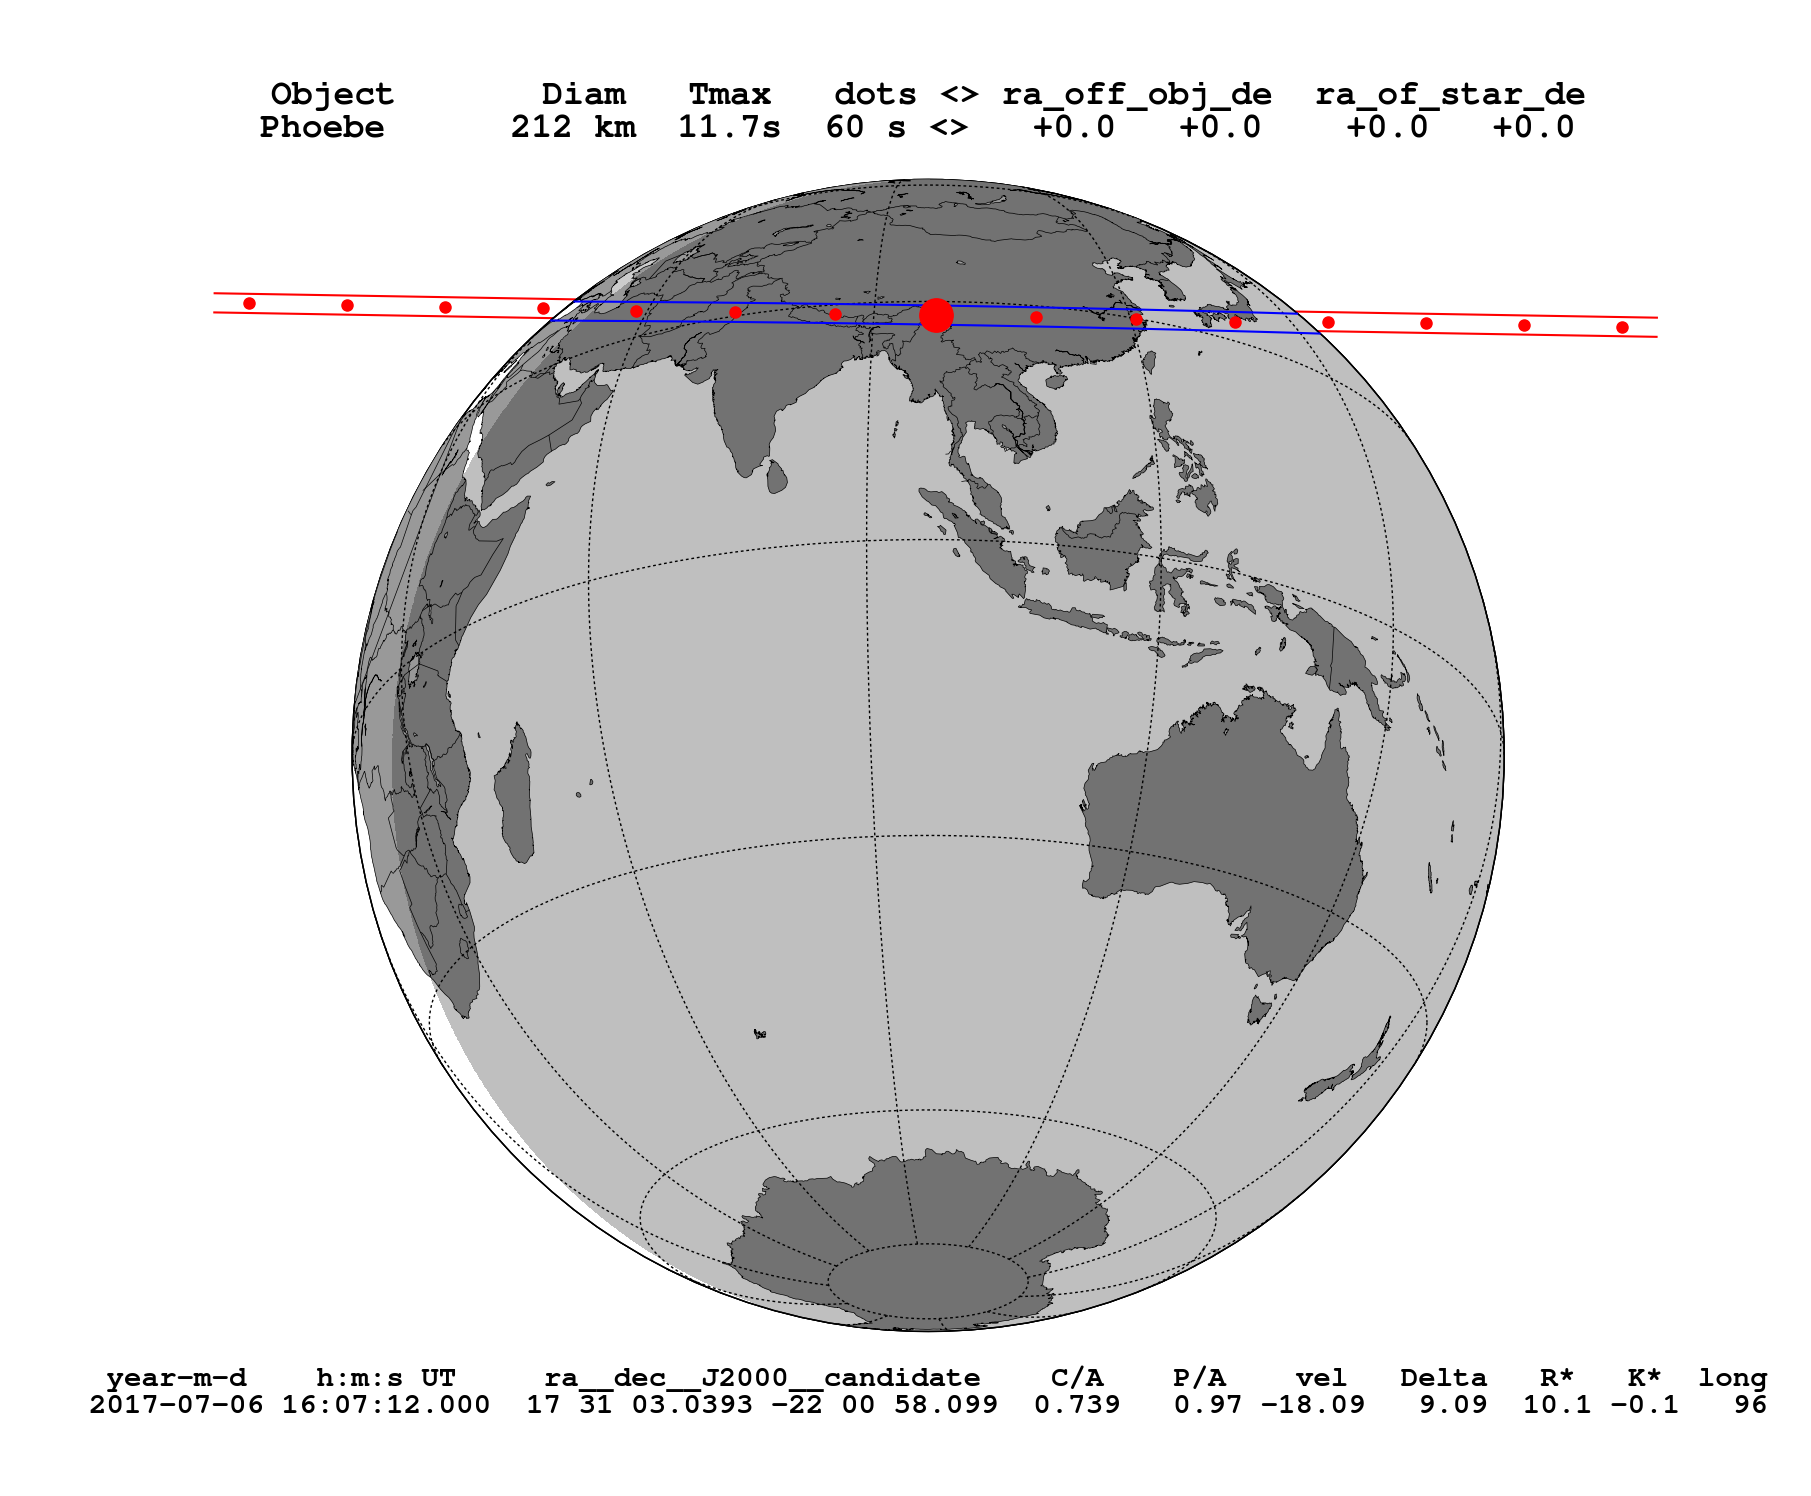
\includegraphics[width = 16.0cm]{figuras/Phoebe_2017-07-06.png}   
\caption{Mapa de Ocultação por Phoebe em 06 de Julho de 2017 observada no Japão.
%The central red dot show the geocentric closest approach of the shadow. The small ones shows the center of the shadow separated by 60s. The lines show the path of the shadow over the Earth. The shadow moves from right to left.
%\textbf{Labels:} Diam: Diâmetro do Objeto; Tmax: Duração máxima do evento para uma observação central; C/A: the geocentric closest approach, in arcseconds; P/A: the satellite position angle with respect to the occulted star at C/A, in degrees; vel: velocity of event in km/s; Delta: Geocentric distance to the occulting object in AU; $R^*$: normalized magnitude to a common shadow velocity of 20 km s$^{-1}$; long: east longitude of subplanet point in degrees, positive towards east.
}
\label{Fig: ocultacao}
\end{centering}
\end{figure}

Até o momento, algumas tentativas foram feitas para observar ocultação por satélites irregulares. Porém, só uma pôde ser observada. Essa foi uma ocultação pelo satélite de Saturno, Phoebe, observada por dois observadores no Japão em 6 de Julho de 2017. É a primeira ocultação por satélite irregular já detectada. A figura \ref{Fig: ocultacao} mostra no mapa a região em que a sombra passou sobre a Terra. As observações já foram recuperadas e estão sendo tratadas.

Essa ocultação e outras que poderão ser observadas serão tratadas por mim. Eu tenho experiência na redução de curvas de luz de ocultação, onde já reduzi curvas de diversas ocultações de Chariklo, Plutão e outros TNOs. Além disso, trabalhei integralmente nas reduções das ocultações de Ceres de 17 de Agosto de 2010 e 25 de Outubro de 2013, inclusive ajustando a forma do corpo aos instantes de imersão e emersão das curvas de luz. Esse trabalho foi publicado em \cite{GomesJunior2015-Ceres}.

\section*{Cronograma para o pós-doc}

\indent \indent Como explicado nos capítulos anteriores, o projeto se divide em três etapas: observação e astrometria dos satélites irregulares; integração numérica de suas órbitas; e observação de ocultações estelares. Para o período de pós-doc de Março de 2018 a Fevereiro de 2019, pretendo realizar as seguintes tarefas:

Observação dos satélites irregulares para astrometria: dentro do programa de observações que o grupo do Rio faz a partir do OPD, os satélites irregulares serão observados. Para os satélites de Júpiter, entre Fevereiro e Setembro de 2018 eles estarão observáveis. Para os satélites de Saturno, entre Março e Outubro. E para os satélites de Netuno, de Maio a Dezembro.

Astrometria: com a publicação da segunda versão do catálogo GAIA em Abril de 2018, todas as observações antigas serão re-reduzidas com esse nova versão. Todo o banco de dados, incluindo as novas imagens, será preparado para uma rápida redução com o novo catálogo. Provavelmente, menos que três meses a partir da publicação serão precisos para o processo de re-redução, considerando as adaptações necessárias para a implementação do GAIA-DR2.

Integração Numérica: como primeira medida, será necessário recuperar na literatura todas as posições publicadas para os objetos estudados. Algumas dessas posições deverão ser convertidas para o Sistema de Referência mais moderno. E todas serão estudadas de forma a se identificar o peso adequado a ser usado na integração numérica. Dentro desse período de um ano, pretendo gerar novas órbitas para os oito satélites irregulares principais de Júpiter e o satélite irregular principal de Netuno, Nereida. Após a re-redução das imagens do OPD ser refeita com o GAIA-DR2, essas órbitas serão atualizadas.  O trabalho de atualização será constante ao longo de todo o período do pós-doc.

Observação de Ocultações Estelares: como mostrado na tabela \ref{Tab: satellite-occultation} existem algumas ocultações previstas para 2018 para os satélites de Júpiter. Esses eventos serão selecionados de acordo com a probabilidade de observação. Porém, devido à recente observação da ocultação por Phoebe, e uma vez que depois de 2018 Phoebe não estará mais cruzando a Via Láctea, uma maior atenção será dada a esse satélite. Uma maior quantidade de eventos detectados permitirá fazer uma composição da forma do satélite em latitudes que não foram observadas pela sonda Cassini. A órbita desse satélite é a melhor conhecida dentre todas os satélites irregulares. O período em que esses eventos poderão ser observados é semelhante ao descrito acima para a observação dos satélites de carátes astrométrico.

Por fim, nesse período, publicarei em revistas científicas de prestígio internacional, a ocultação de Phoebe observada, dentre outras que poderão ser observadas. Publicarei também um novo catálogo de posições astrométricas dos satélites, reduzidas com o GAIA-DR2. Além disso, as órbitas determinadas para esses satélites também serão publicadas.

\bibliography{Referencias}
\bibliographystyle{apalike}


\end{document}
